\section{Coefficients de réflexion et de transmission pour différent potentiel}

Avant de présenter les résultats des coefficients de réflexions et de transmissions pour les différents potentiels,pour lesquels on n'affichera la fonction d'onde que d'une méthode et que d'une seule partie du nombre complexe qui compose celle-ci.


\begin{figure}[!ht]
    \begin{minipage}[c]{.46\linewidth}
        \centering
        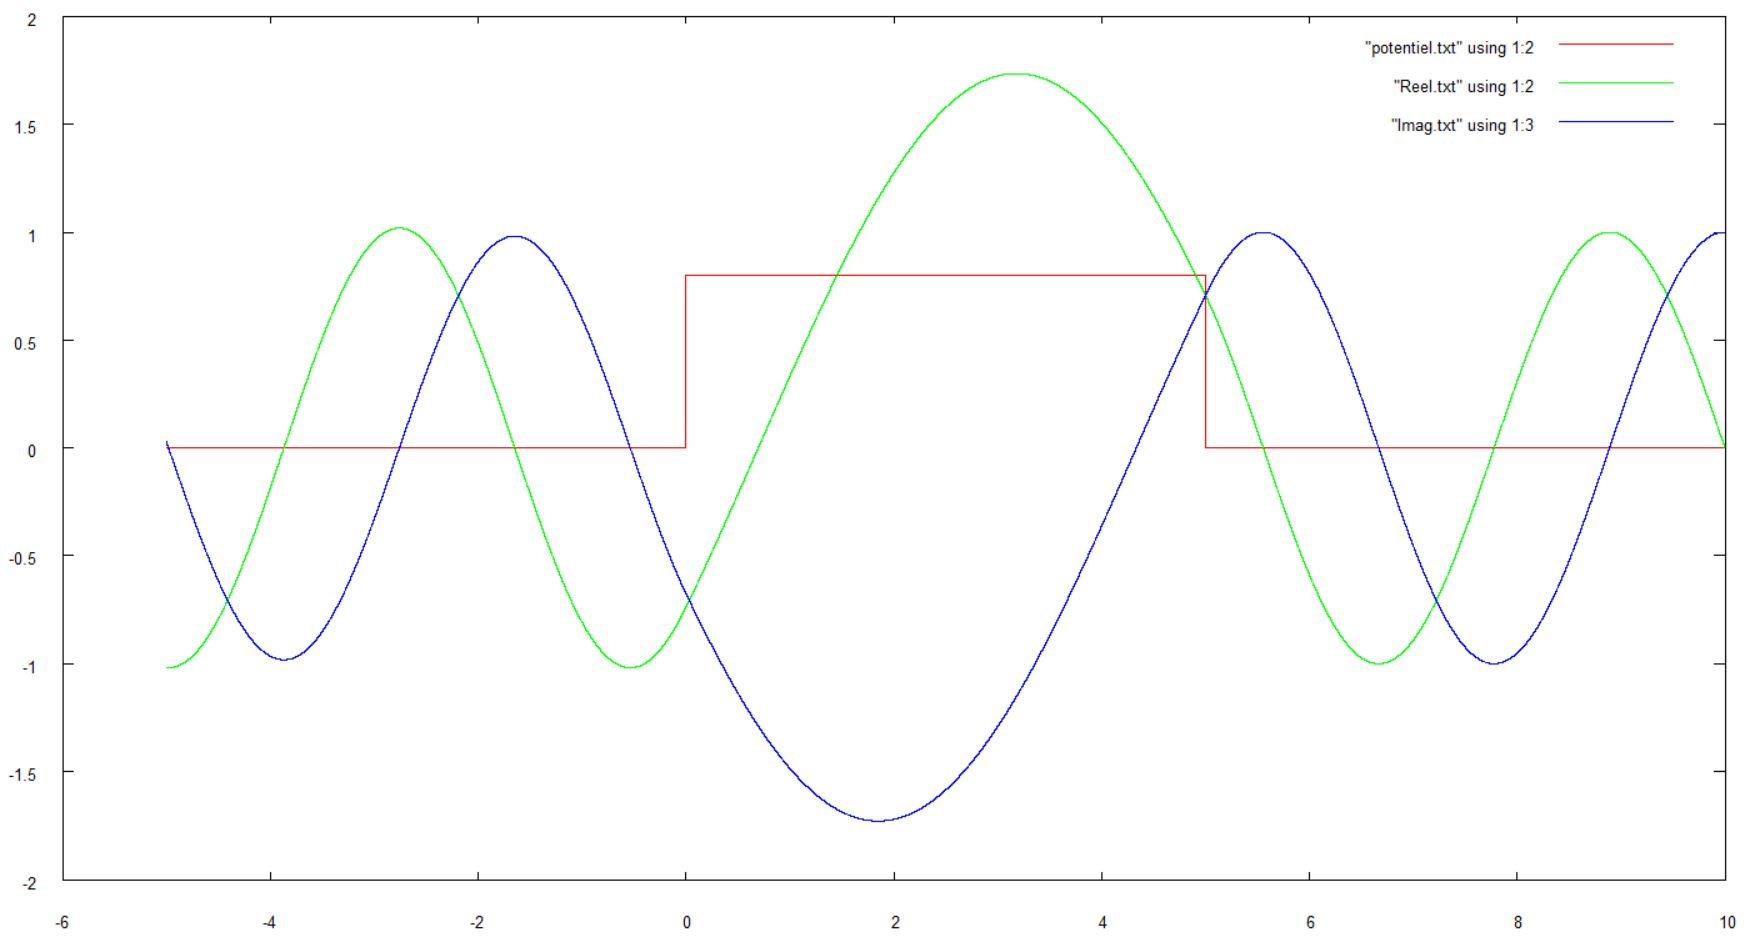
\includegraphics[width=0.9\textwidth]{imag et reel.jpg}
        \caption{Fonction d'onde réel et imaginaire}
    \end{minipage}
    \hfill%
    \begin{minipage}[c]{.46\linewidth}
        \centering
        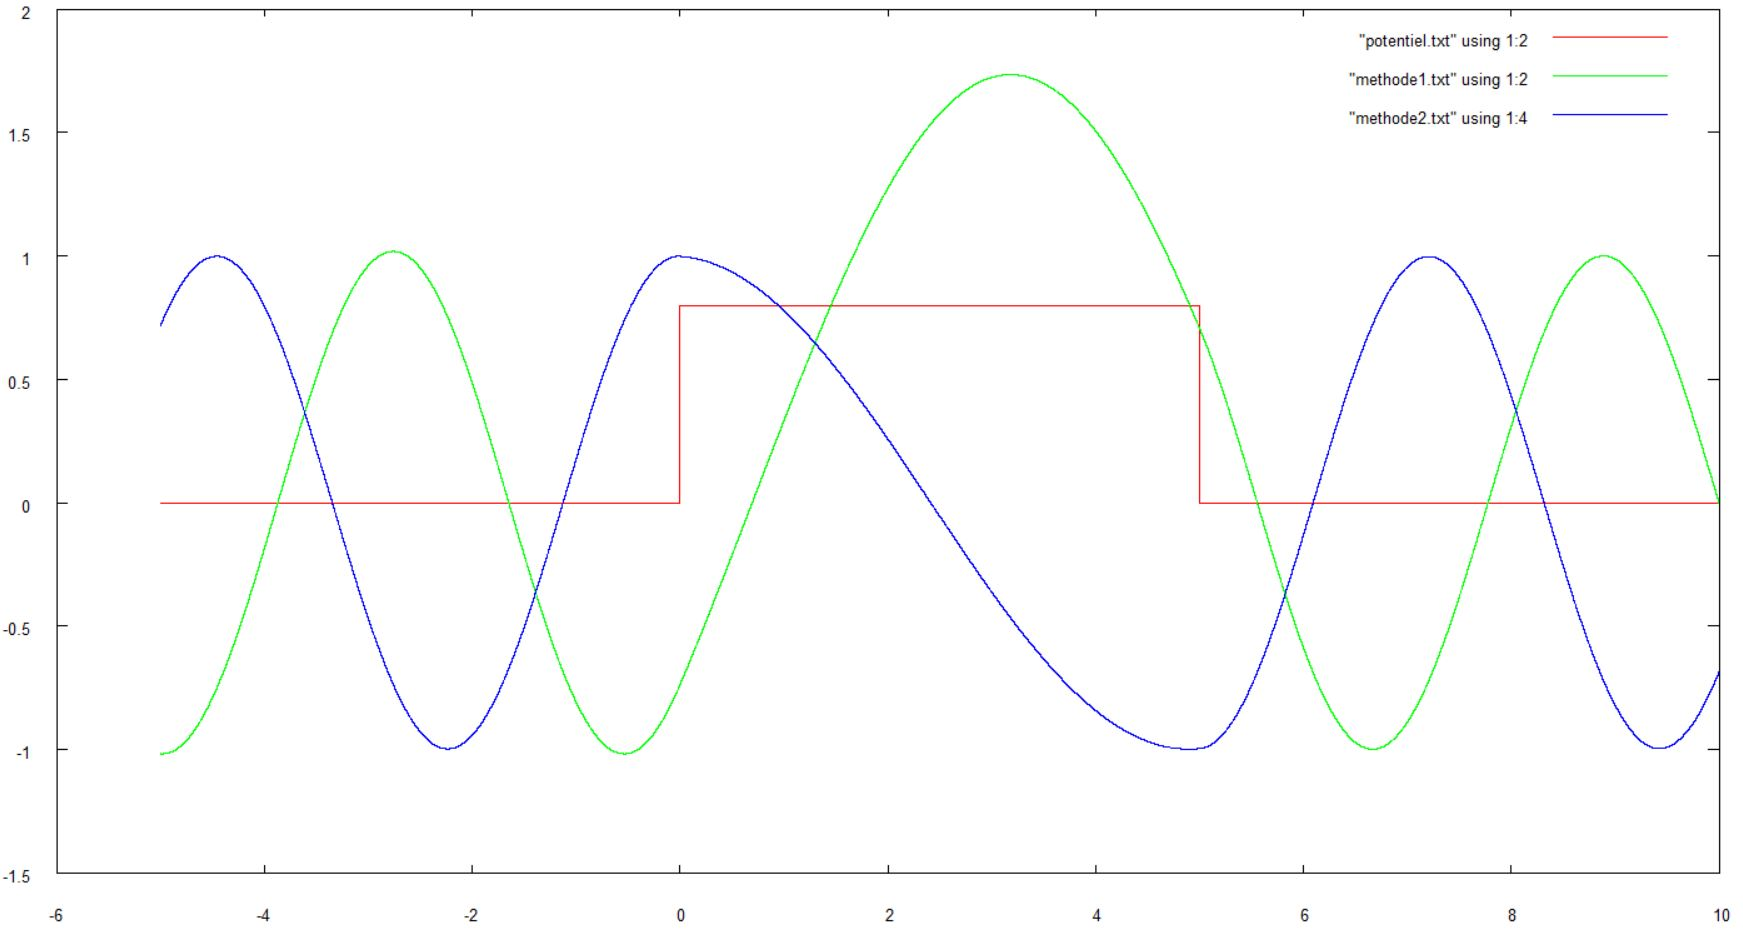
\includegraphics[width=0.9\textwidth]{methode12.jpg}
        \caption{Fonction d'onde réel méthode 1 et 2}
    \end{minipage}
\end{figure}

\subsection{Barrière de potentiel simple}

\begin{figure}[!ht]
    \center
    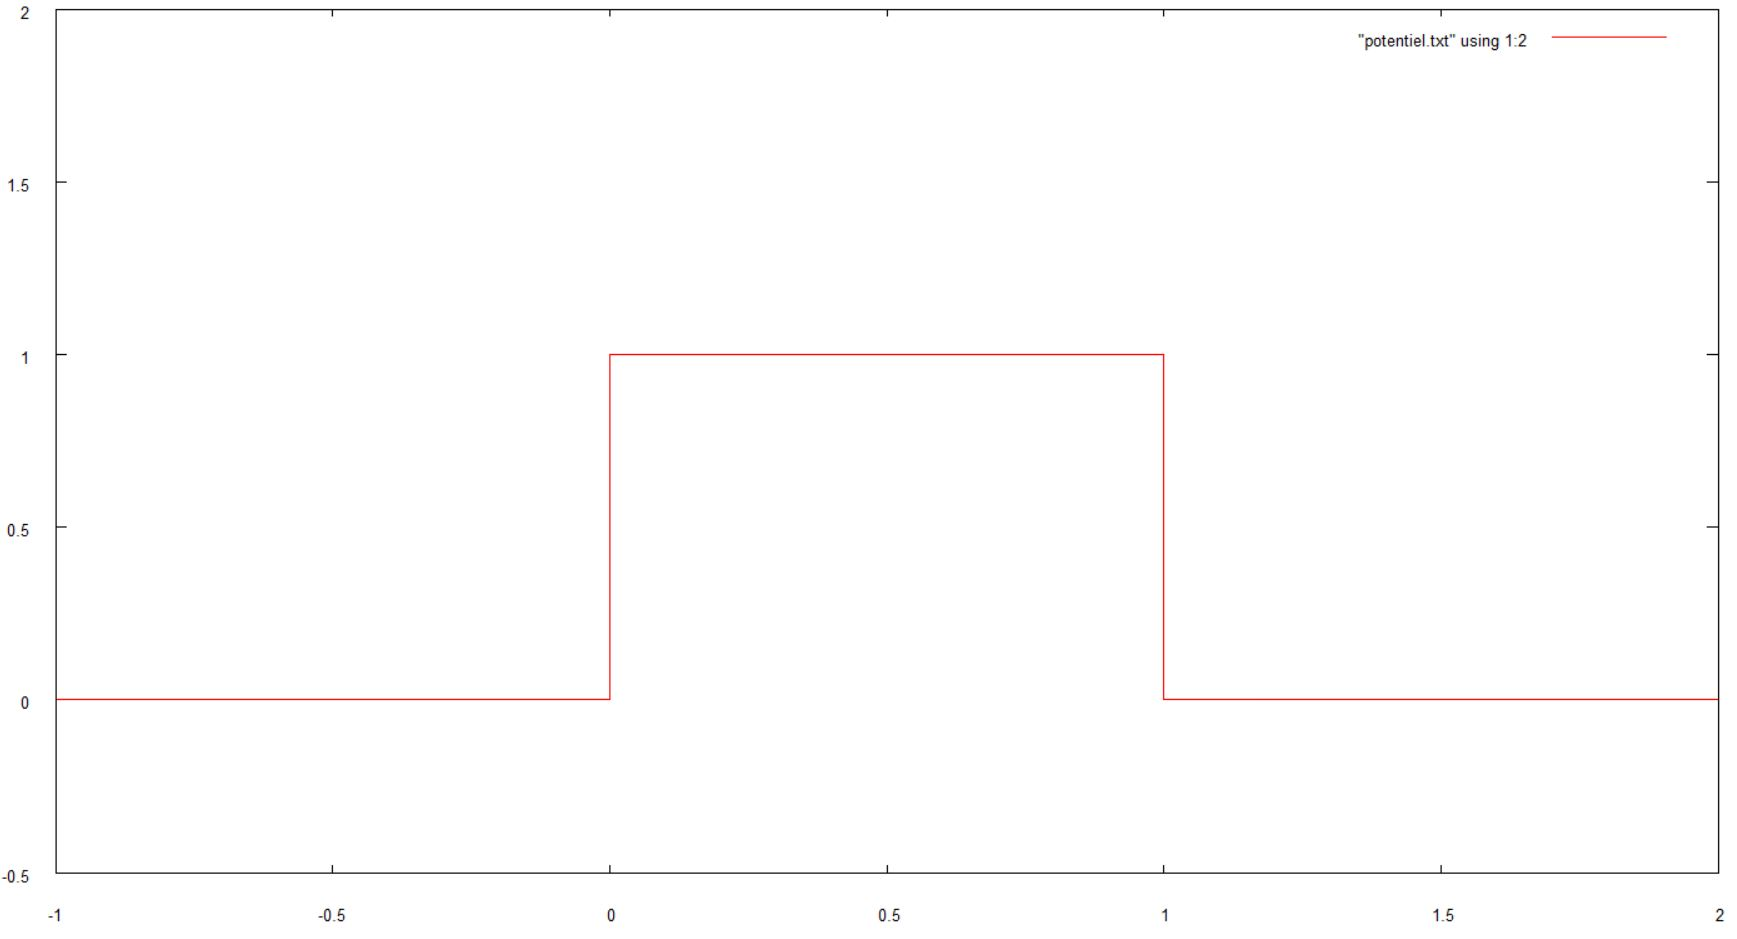
\includegraphics[width=0.4\textwidth]{potentielbarriere.jpg}
    \caption{Barrière de potentiel simple }
    \label{potentielbarriere}
\end{figure}

\begin{table}[!ht]
\centering
Paramètres utilisés  $a=1$,\ $m=1$,\ $V_{0}=1$,\ $N=20000$\\
\begin{tabular}{|l|l|l|}
\hline  Énergie & Coefficient de réflexion  & Coefficient de transmission \\
\hline  0.4 &   0.647581894537856 &  0.352418105437349\\
\hline 1 &  0.333366666342742 & 0.666633334211924\\ 
\hline 1.4 & 0.213549773737718 & 0.786450227124058\\
\hline
\end{tabular}
\caption{Coefficients de réflexion et transmission}
\label{tab3}
\end{table}

\subsection{ 2 Barrières de potentiels simples}

\begin{figure}[!ht]
    \center
    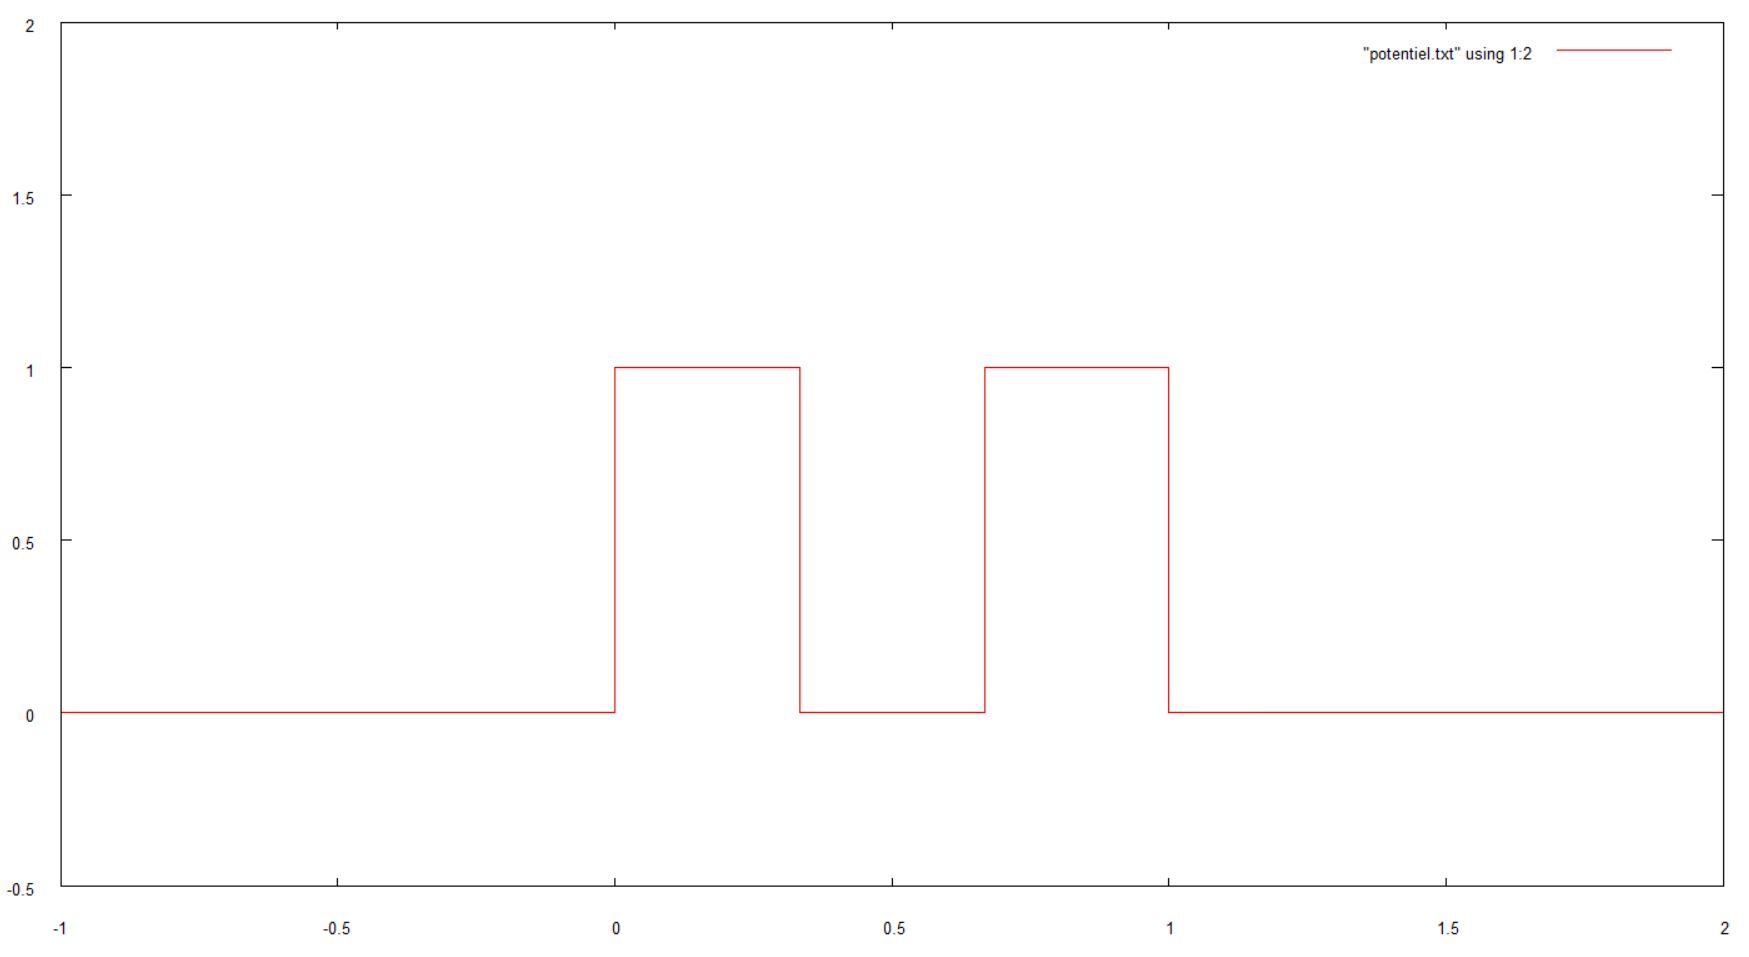
\includegraphics[width=0.4\textwidth]{potentiel2barriere.jpg}
    \caption{2 Barrières de potentiels simples }
    \label{potentiel2barriere}
\end{figure}

\begin{table}[!ht]
\centering
Paramètres utilisés  $a=1$,\ $m=1$,\ $V_{0}=1$,\ $N=20000$\\
\begin{tabular}{|l|l|l|}
\hline  Énergie & Coefficient de réflexion  & Coefficient de transmission \\
\hline  0.4 &  0.398212701243355 &  0.601787299006828\\
\hline 1 & 0.181835356681359 &0.818164643869745\\ 
\hline 1.4 & 0.123418941002287 & 0.876581059844542\\
\hline
\end{tabular}
\caption{Coefficients de réflexion et transmission}
\label{tab4}
\end{table}



\subsection{ 3 Barrières de potentiels simples}
\begin{center}

\end{center}
\begin{figure}[!ht]
    \center
    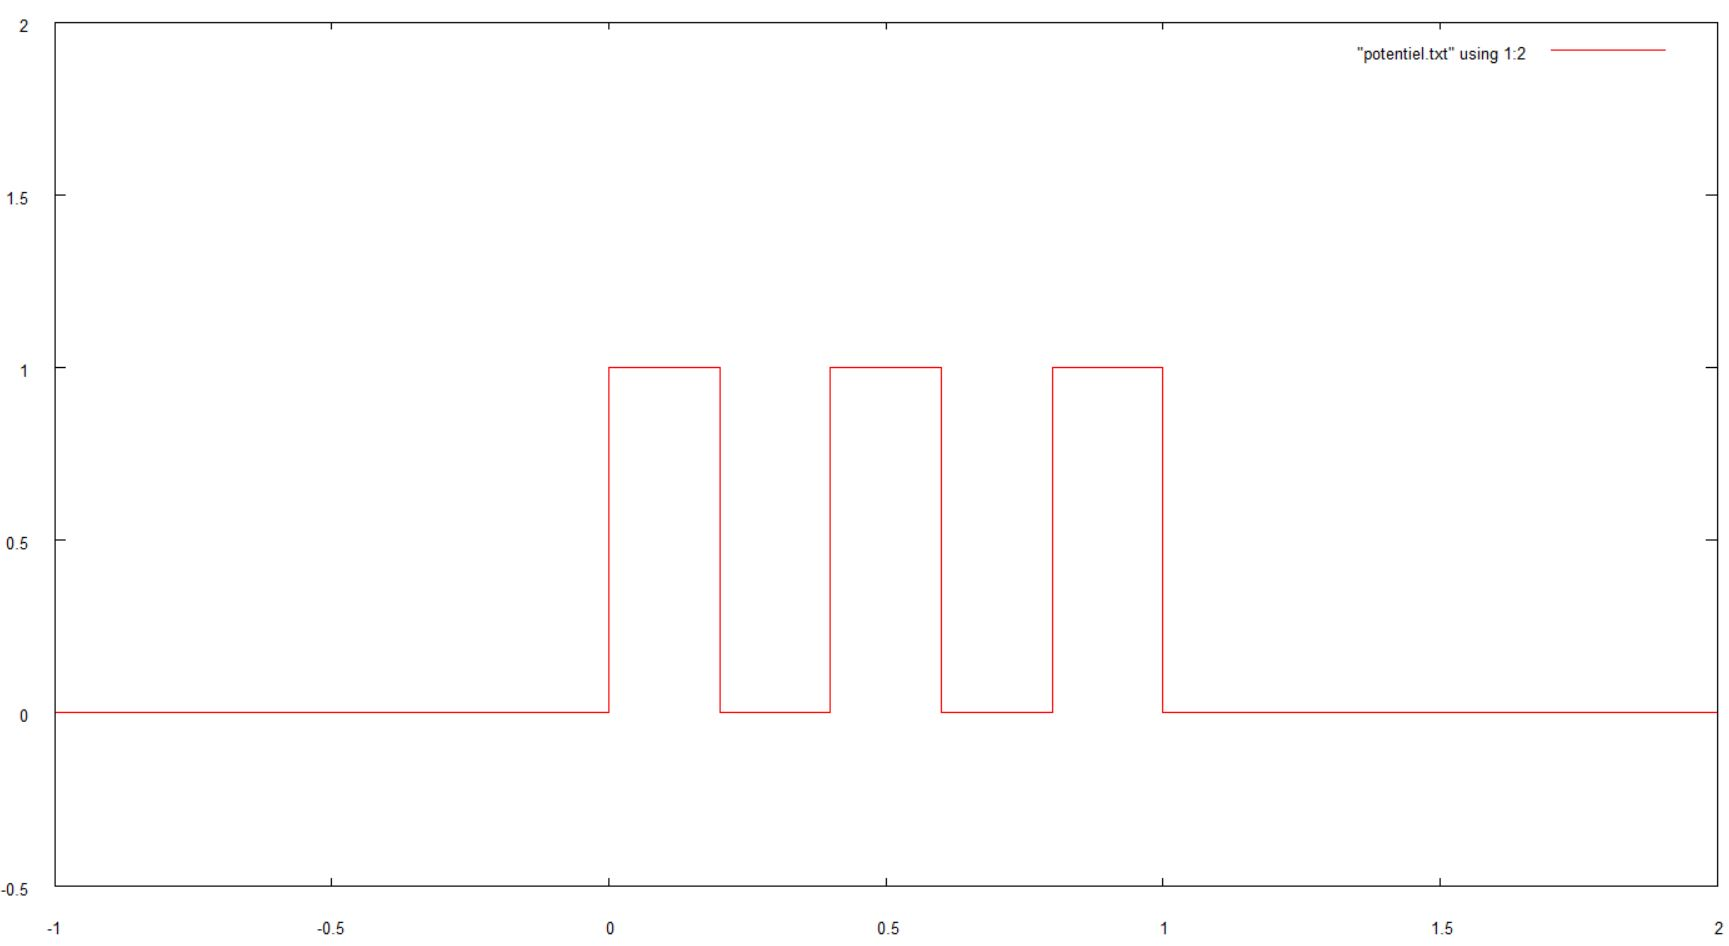
\includegraphics[width=0.4\textwidth]{potentiel3barriere.jpg}
    \caption{ 3 Barrières de potentiels simples}
    \label{potentiel3barriere}
\end{figure}

\begin{table}[!ht]
\centering
Paramètres utilisés  $a=1$,\ $m=1$,\ $V_{0}=1$,\ $N=20000$\\
\begin{tabular}{|l|l|l|}
\hline  Énergie & Coefficient de réflexion  & Coefficient de transmission \\
\hline  0.4 &   0.324948897997792 &  0.675051102149639\\
\hline 1 & 0.0951860743657358 & 0.904813926378733\\ 
\hline 1.4 &0.0456158378203416 & 0.954384163344269\\
\hline
\end{tabular}
\caption{Coefficients de réflexion et transmission}
\label{tab6}
\end{table}

\subsection{Barrière de potentiel gaussienne}
\begin{center}

\end{center}
\begin{figure}[!ht]
    \center
    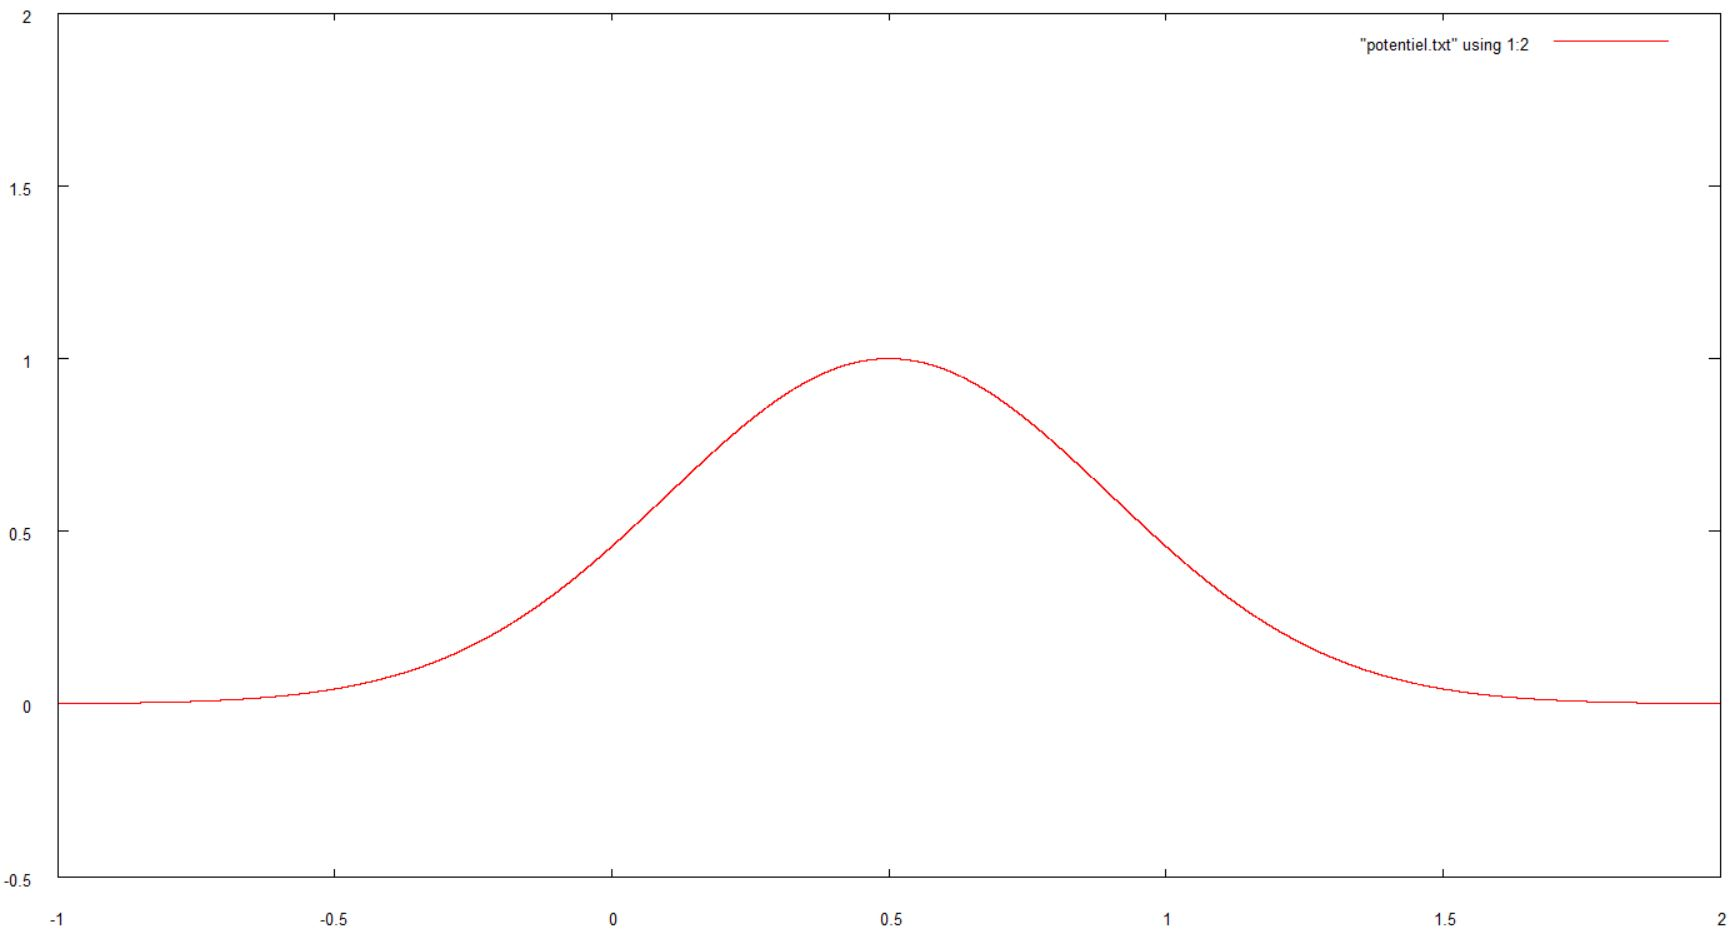
\includegraphics[width=0.4\textwidth]{barrieregaussienne.jpg}
    \caption{ Barrière de potentiel gaussienne}
    \label{barrieregaussiennne}
\end{figure}

\begin{table}[!ht]
\centering
Paramètres utilisés  $a=1$,\ $m=1$,\ $V_{0}=1$,\ $N=20000$\\
\begin{tabular}{|l|l|l|}
\hline  Énergie & Coefficient de réflexion  & Coefficient de transmission \\
\hline  0.4 &  0.0129595728676758 &  0.987040427735775\\
\hline 1 & 0.00462550868263464 & 0.995374492199424\\ 
\hline 1.4 & 0.0030585389705029 & 0.996941462224125\\
\hline
\end{tabular}
\caption{Coefficients de réflexion et transmission}
\label{tab7}
\end{table}

\subsection{Barrière de potentiel triangle}
\begin{center}

\end{center}
\begin{figure}[!ht]
    \center
    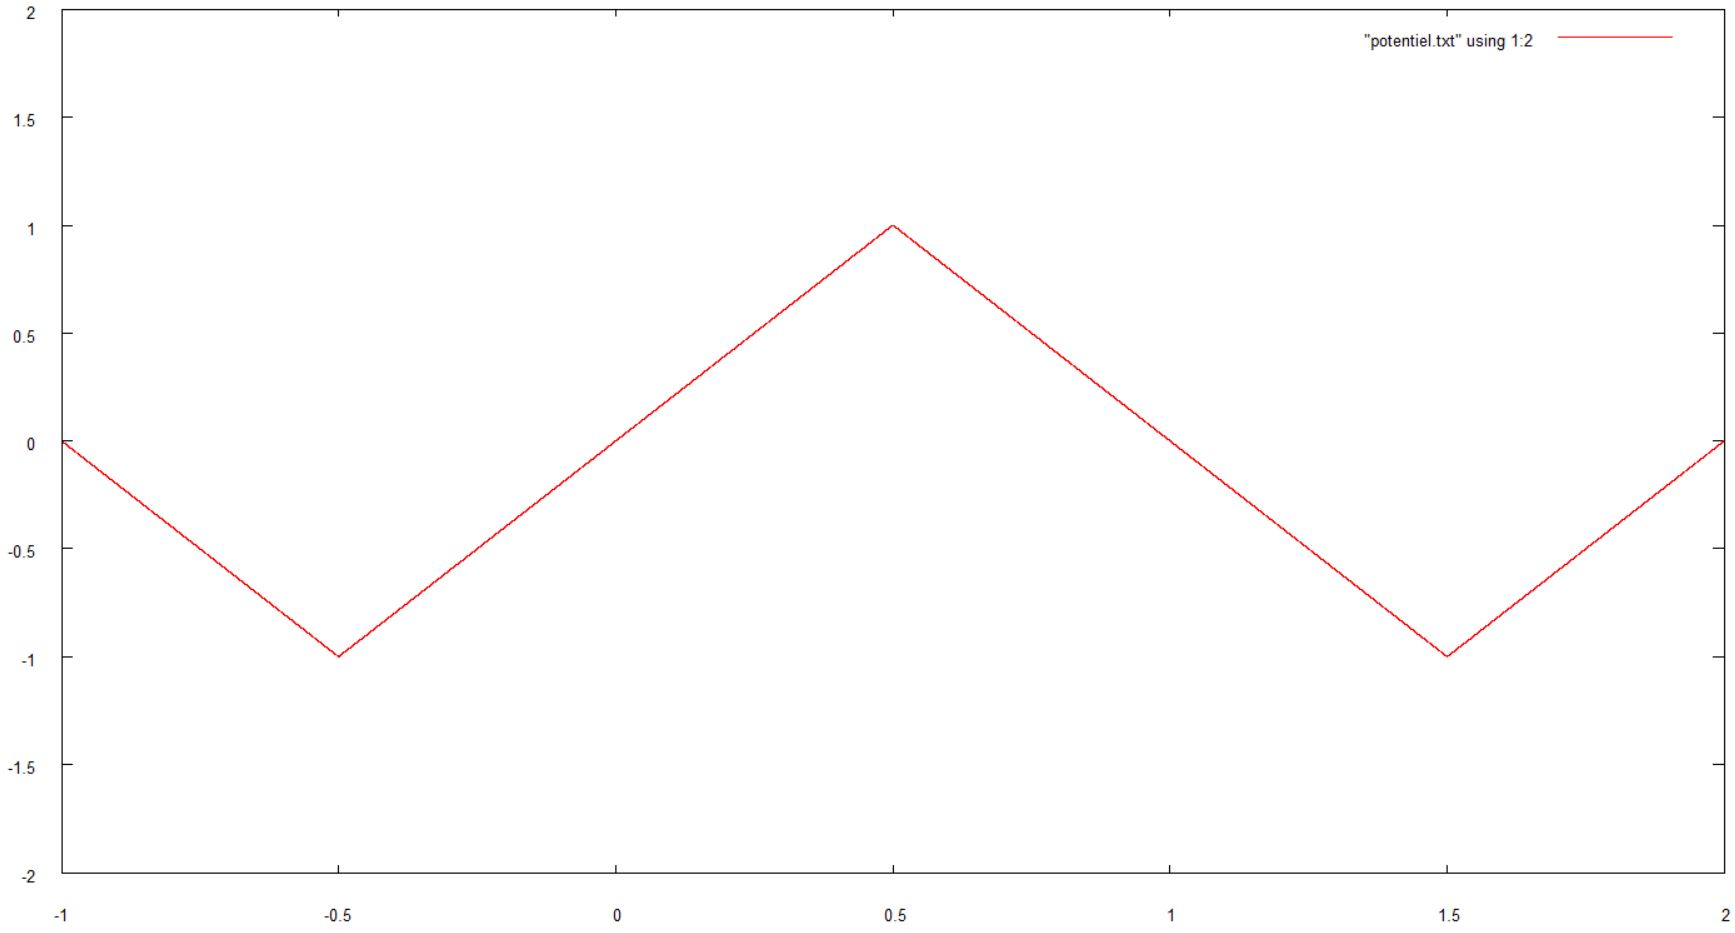
\includegraphics[width=0.4\textwidth]{potentieltriangle.jpg}
    \caption{ Barrière de potentiel triangle}
    \label{potentieltriangle}
\end{figure}

\begin{table}[!ht]
\centering
Paramètres utilisés  $a=1$,\ $m=1$,\ $V_{0}=1$,\ $N=20000$\\
\begin{tabular}{|l|l|l|}
\hline  Énergie & Coefficient de réflexion  & Coefficient de transmission \\
\hline  0.4 & 0.25435128942599 &  0.745648710947624\\
\hline 1 & 0.0947920470348868 & 0.905207953604588\\ 
\hline 1.4 &0.0588079770743296& 0.941192024180452\\
\hline
\end{tabular}
\caption{Coefficients de réflexion et transmission}
\label{tab}
\end{table}


Maintenant que nous avons déterminé les coefficients de transmissions et de réflexions pour les énergie de 0.4 ,1 ,1.4  Hartree.On peut voir que même avec des énergies inférieurs aux potentiels la transmission est non nul. On observe aussi que avec des énergies plus grandes que le potentiel la réflexion devient petite. Nous allons pour la suite nous intéresser à la variation des différents paramètres sur le coefficient de transmission.






